\section{The exterior field and the interior}\label{sec:hair}

\begin{quote}
\textbf{In plain words.} Physicists say that a black hole has no hair: from
outside, nothing can be learnt of what fell into it but its mass, its spin and its charge.
The camera shows that everything is nearly bald. One look at the pull of a
stone tells very little of what is inside it. But a stone, unlike a black hole,
gives itself away to a second look. It trembles with its own heat and it yields
to a push, and in the trembling and the yielding all of its inside can be read,
slowly. It is enough to push it and then weigh it. How much a push tells
depends on its shape. There are pairs of bodies that the simplest squeeze
cannot tell apart and the next one can, and each new shape of squeeze adds one
more number about how the mass is spread between the centre and the surface.
Two pushes, given in either order, tell how the inside is moving. A black hole
trembles and yields too, and tells nothing by it but its temperature.
\end{quote}

The limits of the near field were met one at a time in
Section~\ref{sec:near-field}: an ambiguity, a blur, a count of bits, a tie
broken by heat. They are one subject, and its natural name is hair:
what the field outside a body fixes of its interior. This
section and the three that follow put them together, in the form that
quantum mechanics gives them, and compare a black hole with an ordinary body.

\paragraph{The field at one time.} Outside a body, with no waves coming in from elsewhere,
the field at one time is built from the moments
$Q_h = \int\rho\,h\,\dd V$ of its mass against the functions $h$ that are
harmonic in it, and from the like moments of its flow. A density that has none
of these moments, $\nabla^2\psi/4\pi G$, has no effect on a camera
outside, Eq.~\eqref{eq:split}. This generalizes Newton's shell theorem.
In general relativity still less is fixed at one time. To first
order the constraints fix only the matter's total energy, momentum and angular
momentum and its centre of mass, and the fields of its higher moments can be
cancelled, on that one slice, by a free field added to them
\cite{DonnellyGiddings2017}; in the full theory vacuum data inside a large
enough ball can be joined, across a shell, to a slice of the field of a black
hole, spinning and in general moving, outside it \cite{CorvinoSchoen2006}. The statements of this paper suppose that no such field
has been added (Section~\ref{sec:one-pixel}).

\paragraph{The number of bits.} Read on a sphere of radius $R_c$ about a
body of radius $R$, the multipole of degree $\ell$ is weaker than the monopole
by $(R/R_c)^\ell$, and there are $2\ell + 1$ of each. If the monopole is read at
the signal-to-noise ratio $\SNR$, the argument that gave
Eq.~\eqref{eq:capacity} gives, for the whole body at one time,
\begin{equation}\label{eq:hair-bits}
\begin{gathered}
H \approx \frac{1}{\ln 2}\left[\frac{L^3}{3\Lambda^2} + \frac{L^2}{2\Lambda}\right],\\
L = \ln\SNR, \qquad \Lambda = \ln\frac{R_c}{R}
\end{gathered}
\end{equation}
bits, whose leading term is that of Eq.~\eqref{eq:capacity} for a camera close
to the surface, and is the $\varepsilon$-entropy of the harmonic functions
between the two spheres, the number of bits that fix one of them to the
accuracy $\varepsilon = 1/\SNR$ \cite{KolmogorovTikhomirov1959,SkibaZahariuta2000}. From a distance of three of its radii, a camera with $\SNR = 10^6$ reads
$1200$ bits of a body, and at the ceiling of
Section~\ref{sec:near-field}, $10^{70}$, it reads $1.7\times10^6$: two hundred
kilobytes, for a person watched for the age of the universe. A black hole has
less. All the moments of its field are fixed by its mass and its spin
\cite{Hansen1974}, which with its place make seven numbers in the frame in
which it is at rest (its velocity adds three, as any body's does): at most
$7\log_2\SNR$ bits, $140$ at $10^6$ and $1600$ at $10^{70}$, whatever its
size. A neutron star is nearly as bald, its moment of inertia, its quadrupole
and its yielding to a tide being tied to one another, to about one per cent,
whatever it is made of \cite{YagiYunes2013}. Having no hair is the end of a scale on which every body
lies, and the scale is short. Between a person and a black hole there is a
factor of nearly nine in what gravity can tell at $\SNR = 10^6$, and of a thousand at
that ceiling (Fig.~\ref{fig:hair}(b)).

\begin{figure*}
\centering
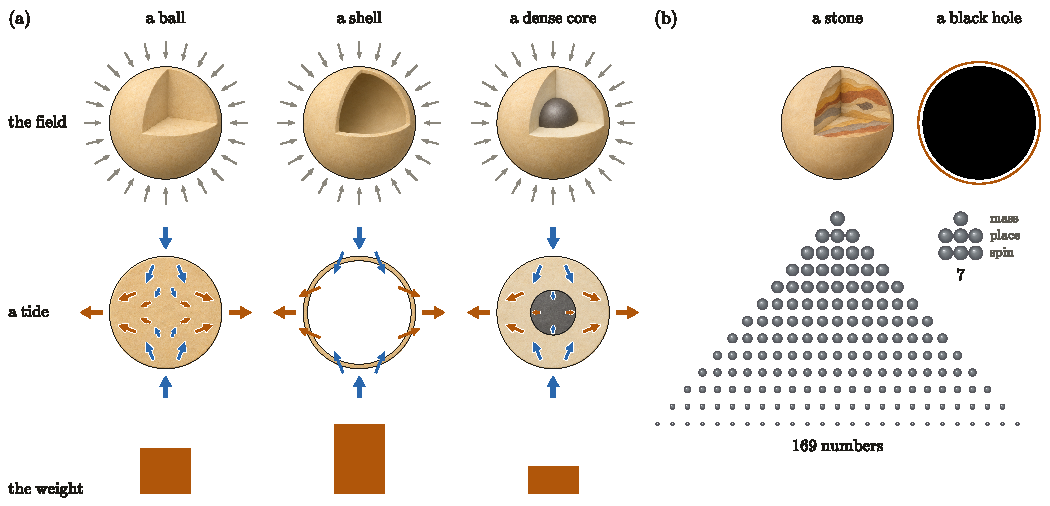
\includegraphics[width=\textwidth]{figures/hair.pdf}
\caption{What the exterior field determines. (a) Three bodies of one size and one mass: a
uniform ball, a shell whose skin is eight per cent of its radius thick, and a
ball of light rock whose core, of $0.4$ of its radius, holds half the mass.
The field: outside, the pull of the three is the same at any one time (grey
arrows). A tide: an
impulsive tide of potential proportional to $x^2 - y^2$ gives each part an
impulse along
$(x, -y)$ and in proportion to its distance from the $z$ axis, outward near one
axis (orange) and inward near the other (blue), drawn on sections of the
three. The weight: the energy each gains, Eq.~\eqref{eq:push}, is proportional to
its $\int\rho\,r^2\,\dd V$, which is $0.60$, $0.92$ and $0.37\,MR^2$ (bars).
(b) The numbers that the field outside carries, a bead for each. A stone read
at $\SNR = 10^6$ from three of its radii shows the $169$ moments of degree
twelve and below, the $2\ell + 1$ of each degree in a row, each bead's area in
proportion to the bits it holds, about $1200$ in all,
Eq.~\eqref{eq:hair-bits}; a black hole at rest shows seven. The cutaway bodies and
the stone's layers are pictures.}\label{fig:hair}
\end{figure*}

\section{Newton's theorem at second order}\label{sec:second-order}

\begin{quote}
\textbf{In plain words.} Newton showed that a hollow shell and a solid ball of
the same weight pull alike on everything outside them. That is true of the
pull. It is not true of what the pull does next. A mass that flies past a body
pulls harder on its near parts than on its far ones and leaves it ringing, and
the energy of the ringing is taken from the mass's own motion, which ends a
little slower. How much slower depends on where the mass inside the body lies.
From the amounts lost on all the ways of missing the body, its inside can be
drawn.
\end{quote}

The ambiguity of Section~\ref{sec:hair} is that of Newton's shell theorem, and
the theorem holds to first order only. The pull of a body on a mass outside it
is of first order in that mass, and holds the harmonic moments; what the body
does in reply, and so what the mass gains or loses, is of second order. The
readings of this section are of second order: a variance of the field, a
response to a second mass, or an energy exchanged with one. They have no null
space.

\paragraph{The field at two times.} A second reading, a moment later, does not
repeat the first, because the moments change. For matter whose forces do not depend on
velocity, with $Q_h = \sum_a m_a h(\mathbf x_a)$ and the rate of change
$\dot Q_g = \tfrac12\sum_a(\mathbf p_a\cdot\nabla g + \nabla g\cdot\mathbf p_a)$
of another, where $\mathbf p_a$ are the momenta, the two do not commute:
\begin{equation}\label{eq:hair-commutator}
[\,Q_h,\,\dot Q_g\,] = i\hbar\int\rho\,\nabla h\cdot\nabla g\,\dd V ,
\end{equation}
and the Poisson bracket of classical mechanics has the same form. The
right-hand side appears elsewhere. In classical thermal
equilibrium $\langle\dot Q_h\dot Q_g\rangle$ is $k_BT$ times it,
Eq.~\eqref{eq:thermal-moment}. It is the whole weight of the response to an
applied tide,
Eq.~\eqref{eq:sum-rule}. And far above every frequency at which
the body can respond, the moment $Q_h$ follows a tide that acts on $Q_g$ as
\begin{equation}\label{eq:dust}
\chi_{hg}(\omega) \to -\frac{1}{\omega^2}\int\rho\,\nabla h\cdot\nabla g\,\dd V ,
\end{equation}
which is the response of dust: driven faster than its bonds can act, every body
responds as a cloud of free mass, as every atom responds to an X-ray as a cloud
of free electrons.

The right-hand side is not a harmonic moment. For $h$
and $g$ harmonic it is the moment of the density against
$\nabla h\cdot\nabla g$, and such products are enough to build any function.
Take $h_\pm = e^{\boldsymbol\zeta_\pm\cdot\mathbf x}$ with
$\boldsymbol\zeta_\pm = \tfrac12(i\boldsymbol\xi \pm \boldsymbol\eta)$, where
$\boldsymbol\eta$ is perpendicular to $\boldsymbol\xi$ and as long. Both are
harmonic, since $\boldsymbol\zeta_\pm\cdot\boldsymbol\zeta_\pm = 0$, and
\begin{equation}\label{eq:calderon}
\int\rho\,\nabla h_+\cdot\nabla h_-\,\dd V
= -\tfrac12\,|\boldsymbol\xi|^2\int\rho\,e^{i\boldsymbol\xi\cdot\mathbf x}\,\dd V :
\end{equation}
the data at two times are the Fourier transform of the density. This is
Calder\'on's argument \cite{Calderon1980}, made for the problem of finding the
conductivity inside a body from currents and voltages at its surface. The
present problem is that one in its linearized form, with density in place of conductivity, and
here, in Newton's theory, the linear form is exact. The null space of
Eq.~\eqref{eq:split} is therefore a property of a reading at one time, not of
gravity. The
nugget, its flush and its skin (Fig.~\ref{fig:same-outside}) have the same
exterior field at any instant, and are told apart as soon as they are warm or
a tide is applied.

\paragraph{The two readings as one transform.} For a flat camera the relation
between the two readings can be written out. Let the camera lie in the plane
$z = 0$ and the scene beneath it, at depths $z > 0$. The harmonic functions
that decay into the scene are
$h_{\mathbf k} = e^{i\mathbf k\cdot\mathbf a - |\mathbf k|z}$, with $\mathbf a$
the position across the camera and $\mathbf k$ a wave vector in its plane.
Write the transform of the scene, Fourier across and Laplace in depth, as
\begin{equation}\label{eq:scene-transform}
\tilde\rho(\mathbf K, \kappa) = \int\rho(\mathbf a, z)\,
e^{i\mathbf K\cdot\mathbf a - \kappa z}\,\dd^2a\,\dd z .
\end{equation}
The moment of $h_{\mathbf k}$, and the right-hand side of
Eq.~\eqref{eq:hair-commutator} for two such functions, are then
\begin{equation}\label{eq:cone}
\begin{gathered}
Q(\mathbf k) = \tilde\rho(\mathbf k, |\mathbf k|),\\
\int\rho\,\nabla h_{\mathbf k}\cdot\nabla h_{\mathbf k'}\,\dd V
= \tfrac12\,(\kappa^2 - K^2)\,\tilde\rho(\mathbf K, \kappa),
\end{gathered}
\end{equation}
with $\mathbf K = \mathbf k + \mathbf k'$, $K = |\mathbf K|$ and
$\kappa = |\mathbf k| + |\mathbf k'| \ge K$. A reading at one time holds the
transform on the cone $\kappa = K$. Readings at two times hold it inside the
cone (Fig.~\ref{fig:two-readings}(a)), multiplied by half of $\kappa^2 - K^2$, which is the Laplacian in these
variables and vanishes on the cone. A density of the null space,
$\nabla^2\psi/4\pi G$, has the transform $(\kappa^2 - K^2)\,\tilde\psi/4\pi G$:
nothing on the cone, and inside it exactly what the second reading holds. Each
point inside the cone is reached by every pair $(\mathbf k, \mathbf k')$ on an
ellipse with foci at $0$ and $\mathbf K$ (Fig.~\ref{fig:two-readings}(b)), and
all of them agree when the
forces within the scene do not depend on velocity. Each relation is known
apart from the other. The first is the formula of potential-field geophysics
\cite{Parker1973}. That a source whose transform is a multiple of
$\kappa^2 - K^2$ is local, and leaves the multipoles and the distant field as
they were, is known in the same variables for the stress tensors of compact
bodies \cite{GoldbergerRothstein2006a,BianchiEtAl2025}. The second is the
relation of optical tomography in a half space, with a source and a detector
on the surface in the place of the two tides
\cite{MarkelSchotland2001,ArridgeSchotland2009}, where the many pairs that
reach one point are averaged to steady the inversion. That problem has no
reading without a source, and so no cone.

\begin{figure}
\centering
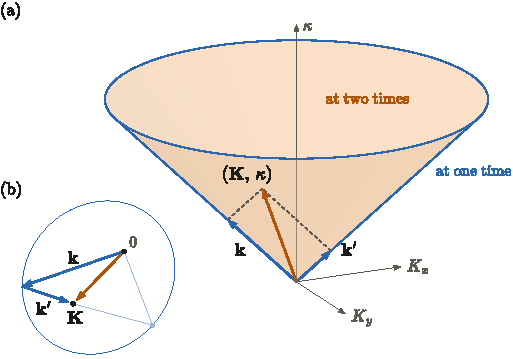
\includegraphics[width=\columnwidth]{figures/two-readings.pdf}
\caption{The two readings as one transform. (a) The space of the scene's
transform, Eq.~\eqref{eq:scene-transform}: $\mathbf K$ across a flat camera,
and the rate of decay with depth, $\kappa$. A reading at one time holds the
transform on the cone $\kappa = K$ (blue outline); readings at two times hold
it inside (orange). The harmonic functions $h_{\mathbf k}$ and
$h_{\mathbf k'}$ are two points of the cone, drawn here on its outline, and
the second reading made with them holds the transform at their sum,
$(\mathbf k + \mathbf k',\,|\mathbf k| + |\mathbf k'|)$, which lies inside.
(b) The plane of $\mathbf K$ seen from above. The same point
$(\mathbf K, \kappa)$ is reached by every pair with $\mathbf k$ on the ellipse
$|\mathbf k| + |\mathbf K - \mathbf k| = \kappa$, whose foci are $0$ and
$\mathbf K$: the pair of (a), and one other (pale).}\label{fig:two-readings}
\end{figure}

\paragraph{Stability.} Each of $h_\pm$ grows to $e^{|\boldsymbol\xi|R/2}$ across
a body of radius $R$, and the camera must build them from multipoles that reach
it weakened by $(R/r)^\ell$ at each degree, so detail of size
$2\pi/|\boldsymbol\xi|$ costs exponentially in sensitivity, as in
Eq.~\eqref{eq:evanescent}. This is a known property of Calder\'on's
problem, whose stability, for conductivities bounded beforehand, is logarithmic
and cannot be better \cite{Alessandrini1988,Mandache2001}. Readings at two
times remove the ambiguity and keep the blur.

\paragraph{An impulsive tide and a weighing.} The second reading can be of a single
number. Let a tide act on the body impulsively: masses outside make, for
an instant, the potential $-\epsilon\,g(\mathbf x)\,\delta(t)$, with $g$
harmonic in the body, and each part of it, of mass $m$, receives the impulse
$\epsilon m\nabla g$ where it stands. For matter whose forces do not depend on velocity the energy
gained is
\begin{equation}\label{eq:push}
\Delta E = \epsilon\,\dot Q_g + \frac{\epsilon^2}{2}\int\rho\,|\nabla g|^2\,\dd V ,
\end{equation}
exactly in Newton's mechanics; it is the sum rule of Eq.~\eqref{eq:sum-rule}
in time instead of frequency, and it holds of the operators of quantum
mechanics, where the impulse is $e^{i\epsilon Q_g/\hbar}$. Energy has weight:
the mass that the monopole of the body's field reports rises by $\Delta E/c^2$, and
an isolated body keeps the gain until it is read. Impulses of both signs,
given to two copies of the body prepared alike, and two weighings give $\int\rho\,|\nabla g|^2\,\dd V$ and,
separately, $\dot Q_g$. The first, with the impulses taken in pairs, is the left-hand
side of Eq.~\eqref{eq:calderon}: sixteen weighings for each Fourier component of the
density. The second then gives the motion. For a body of $N$ parts the
gradients of harmonic functions at their $N$ places can be chosen at will, so
that, once the places are known from the density, enough impulses give every
momentum (Appendix~\ref{app:proofs}). A ball and
a shell of the same weight and the same exterior field gain energy from the
same quadrupolar impulsive tide in the ratio three to five
(Fig.~\ref{fig:hair}(a), where the shell has some
thickness). Only the weight has been read, the one
number that Gauss's law carries to any distance.

The measurement is far beyond reach. An impulse that changes velocities by
$\Delta v$ raises the weight by about $\tfrac12(\Delta v/c)^2$ of itself, five
parts in $10^{41}$ for $\Delta v = 3\times10^{-12}\,\mathrm{m\,s^{-1}}$, which the
tide of a tonne a metre away gives the edge of a body a metre across in fifty
microseconds, far less time than any such mass could be brought up and taken
away in; fine detail costs
exponentially in sensitivity, as before; the impulse must be over before the body can respond,
which requires that the body's own motions be slow compared with light; and
Eq.~\eqref{eq:push} is the first order in $1/c^2$, not the whole theory.

\paragraph{A mass that passes.} Neither the weighing nor the contrived instant
is needed. Held for an instant at a point $\mathbf y$ outside the body, a
mass $\mu$ is the impulsive tide of profile
$1/|\mathbf x - \mathbf y|$, and by Eq.~\eqref{eq:push} a body at rest gains
in proportion to $\int\rho\,|\mathbf x - \mathbf y|^{-4}\,\dd V$. The kernel
of the field, $1/|\mathbf x - \mathbf y|$, is harmonic; that of the energy is
not, and its values at points outside the body fix the density
(Appendix~\ref{app:proofs}).

Let the mass now fly past the body on a straight line at the speed $V$, fast
enough that the parts of the body do not move meanwhile, and let $\mathbf b$
be the point where its path crosses the plane through the body at right angles
to it. A part of the body that lies over the point $\mathbf s$ of that plane
receives the velocity $C(\mathbf b - \mathbf s)/|\mathbf b - \mathbf s|^2$,
with $C = 2G\mu/V$, wherever it lies along the path: the impulsive tide of
profile $-\ln|\mathbf s - \mathbf b|$, which is harmonic in a body that the
path misses. By Eq.~\eqref{eq:push} the body gains
\begin{equation}\label{eq:pass}
\Delta E(\mathbf b) = \frac{C^2}{2}\int
\frac{\Sigma(\mathbf s)}{|\mathbf b - \mathbf s|^2}\,\dd^2s ,
\end{equation}
with $\Sigma$ its mass per area, projected along the path. This is the heating
of a star cluster by a passing mass, in the impulse approximation of stellar
dynamics \cite{Spitzer1958,BanikVanDenBosch2021}. What the body gains the passing mass has lost,
and it leaves slower by $\Delta E/\mu V$: nothing is weighed, and the speed of
light does not enter. The losses on the paths that miss the body give every
moment of $\Sigma$, and paths in the directions of one great circle give the
density (Appendix~\ref{app:proofs}). The deflection of the passing mass is of
first order and holds only the moments of $\Sigma$ against the powers of
$x + iy$: it is the shell theorem in the plane. For a round body the integral
of Eq.~\eqref{eq:pass} is
$M/b^2 + \tfrac23\int\rho\,r^2\,\dd V/b^4 + \tfrac{8}{15}\int\rho\,r^4\,\dd V/b^6$
and so on, of which the first term is the recoil of the whole body. A thin shell
of mass $M$ and radius $R/\sqrt2$, and a point of mass $M/2$ at the centre of
a shell of radius $R$ that holds the other half, are alike in the first two
terms. They differ by
$30\%$ in the internal energy that one pass at $b = 1.5R$ leaves in them, and
by $MC^2R^4/15b^6$ far away (Fig.~\ref{fig:passing}). The loss is as far beyond reach as the weighing:
a tonne that passes a metre from the edge of a steel ball a metre across at
$44\,\mathrm{km\,s^{-1}}$ gives that edge the impulse of the last paragraph,
and leaves with its speed lower by five parts in $10^{33}$.

\begin{figure}
\centering
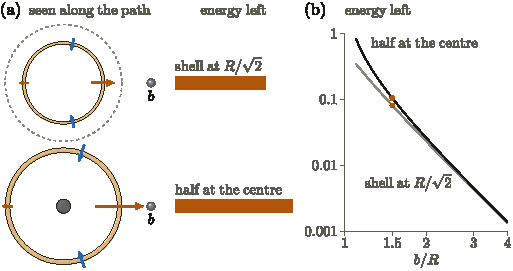
\includegraphics[width=\columnwidth]{figures/passing.pdf}
\caption{A mass that passes. (a) Two bodies with the same field outside,
a thin shell of mass $M$ and radius $R/\sqrt2$ (above) and a point of mass
$M/2$ at the centre of a shell of radius $R$ that holds the other half
(below), seen along the path of a mass that crosses the page at $b = 1.5R$
(the bead).
Arrows: the impulses that parts of each shell receive, less that of the body
as a whole, outward (orange) or inward (blue), at the four places where they
lie along the radius; the mass at the centre receives none. Bars: the internal
energy left in each, $0.080$ and $0.104\,MC^2/2R^2$. (b) That energy against
the distance of the pass, in the same units. The two gain alike from every quadrupolar tide
(Fig.~\ref{fig:ladder}) and are told apart by one pass. The cutaway bodies are pictures, and the skins, the mass at the
centre and the bead are drawn with some size.}\label{fig:passing}
\end{figure}

The pair $h_\pm$ of Eq.~\eqref{eq:calderon} varies in two directions only. Each
is the profile of a wave with flat fronts that travels along the third, and in
general relativity such a wave, arriving all at once with any profile $H$ that
is harmonic across its front, is an exact solution; the field of a particle
without mass is one \cite{AichelburgSexl1971}. A particle of energy $E$ and
momentum $\mathbf p$ that crosses it keeps $E - cp_z$, with $z$ the direction
of the wave, and its momentum across that direction changes by
$(E - cp_z)\nabla H/2c$ \cite{Balasin1997,Steinbauer1998}, so that it
gains the energy
\begin{equation}\label{eq:shock}
\Delta E = \tfrac12\,c\,\mathbf p_\perp\cdot\nabla H
+ \tfrac18\,(E - cp_z)\,|\nabla H|^2
\end{equation}
at any speed, light included. This is Eq.~\eqref{eq:push} without the
restriction to slow matter. Summed over a body, the first term has either
sign, so one wave can take energy from what it crosses. The part that is even
in the wave cannot. With $E_\pm$ the energy of the body after the wave and
after its reverse, and $E_0$ its energy with no wave,
\begin{equation}\label{eq:shock-even}
E_+ + E_- - 2E_0 = \tfrac14\int|\nabla H|^2\,\mathcal N\,\dd^2x_\perp \ge 0 ,
\end{equation}
where $\mathcal N(\mathbf x_\perp)$ is the energy, less $c$ times the momentum along
the wave, that crosses the front at $\mathbf x_\perp$: the integral of
$T_{\mu\nu}k^\mu k^\nu$ along the null ray through that point, with $k^\mu$
the wave's direction, which is also the generator of the displacement that
the wave gives to whatever crosses it
\cite{CasiniTesteTorroba2017,CordovaShao2018}. For the rest mass the mean
square of $\nabla H$ is replaced by its variance over the body, which cannot
be negative either (Appendix~\ref{app:proofs}). Pairs of such waves therefore read the Fourier
transform, at $\boldsymbol\xi$, of $\mathcal N$: a projection along the wave's path, as
in X-ray tomography, and waves from all directions give the integrals of the
stress tensor along every ray of light. What those integrals leave
undetermined is known \cite{KrishnanSenapatiVashisth2020}. A stress tensor of
the form $(\partial_\mu\partial_\nu - \eta_{\mu\nu}\Box)\phi$ has none; for a
body at rest it adds $\nabla^2\phi$ to the density of energy, with stresses to
match, and it is excluded when the stresses are small beside $\rho c^2$.
The particle without mass is the passing mass of Eq.~\eqref{eq:pass} at the
speed of light. Its wave has the profile
$H = -(8Gp/c^3)\ln|\mathbf x_\perp - \mathbf b|$, with $p$ its momentum, which
is harmonic across the front wherever its path misses the body, and a body
whose parts are at rest gains
\begin{equation}\label{eq:massless-pass}
\Delta E(\mathbf b) = \frac{8G^2p^2}{c^6}\int
\frac{\mathcal N(\mathbf s)}{|\mathbf b - \mathbf s|^2}\,\dd^2s .
\end{equation}
For slow matter $\mathcal N = \Sigma c^2$, and this is Eq.~\eqref{eq:pass}
with $C = 4Gp/c^2$, twice Newton's value, as for the bending of light. A
particle sent in from infinity and received there thus reads the same
transform of the energy that crosses each point of its front.
For a wave of finite duration Eq.~\eqref{eq:shock} holds when the matter
moves little across the front while the wave passes.

\paragraph{The bits of a second reading.} Read at the points outside a sphere
of radius $R_c$, the energies left by a mass held for an instant hold every
moment $\int\rho\,r^{\ell+2j}Y_\ell\,\dd V$: $(n+1)(n+2)/2$ of them of total
degree $n = \ell + 2j$, where the field at one time has $2n + 1$. The count of
Eq.~\eqref{eq:hair-bits} then grows as the fourth power of $\ln\SNR$ in place
of the cube, a volume's worth of the body against a surface's worth, each
logarithmic. From three radii a body gives $1300$ bits at a signal-to-noise
ratio of $10^6$ and $9.6\times10^6$ at $10^{70}$, against the $1200$ and
$1.7\times10^6$ of the first reading; read on a single sphere, the second
reading gives only as many as the first. The ratio meant is that of the second
reading's own leading term, which for a passing mass is smaller than that of
the first by $2G\mu/bV^2$.

\paragraph{What a tide of a given degree reaches.} A tide made by masses
outside a body is, within it, a sum of harmonic polynomials: of degree two if the
masses are far away, with terms of higher degree as they come near. How much
of the interior is reached depends on that degree. Let the applied profile $g$
be any harmonic polynomial of degree at most $m$, and the moment read, $Q_h$,
any at all. The functions $\nabla h\cdot\nabla g$, against which the density
is then known, span together with the harmonic polynomials exactly the
polynomials $P$ that satisfy
\begin{equation}\label{eq:ladder}
\nabla^{2m}P = 0 .
\end{equation}
In each angular sector these are the radial moments
$\int\rho\,r^{\ell+2j}\,Y_\ell\,\dd V$, with $Y_\ell$ a surface harmonic of
degree $\ell$ and $j < m$, of which a reading at one
time has only $j = 0$. A quadrupolar tide adds one radial moment to every
sector, an octupolar tide the next (Fig.~\ref{fig:ladder}(b)). To leading order in the strength of the tide, no tide of degree $m$ reaches
further, whatever is read, because for harmonic $h$ and $g$
\begin{equation}\label{eq:ladder-identity}
\nabla^{2m}(\nabla h\cdot\nabla g) = 2^m\,
(\partial_{i_1}\!\cdots\partial_{i_{m+1}}h)\,
(\partial_{i_1}\!\cdots\partial_{i_{m+1}}g) ,
\end{equation}
which vanishes when either has degree $m$ or less; that everything allowed by
Eq.~\eqref{eq:ladder} is reached is shown in Appendix~\ref{app:proofs}. The
same structure is known in the problem of finding a conductivity from
currents and voltages at a surface. Linearized about a uniform ball, it is
a triangular system, in which currents of degree up to $m$ give exactly the
first $m$ radial orders of the conductivity in every angular sector
\cite{GardeHirvensalo2025}, as they do in a disc \cite{GardeHyvonen2024}.
Here it is a statement of what an observer with limited tides cannot tell
apart. Two
densities that differ by $\nabla^{2m}\psi$, with $\psi$ confined to the body,
therefore have the same exterior field and the same response to every tide of
degree up to $m$, and differ under a tide of degree $m + 1$; in the variables
of Eq.~\eqref{eq:cone} the difference of their transforms vanishes at the cone
as $(\kappa^2 - K^2)^m$, and that of their second readings as
$(\kappa^2 - K^2)^{m+1}$. The simplest such pair (Fig.~\ref{fig:ladder}(a)) is
a thin shell of mass $M$ and radius $R/\sqrt2$, and a point of mass $M/2$ at the centre of a shell of
radius $R$ that holds the other half. The two have the same exterior field
and the same $\int\rho\,r^2\,\dd V$. An impulsive tide of profile
$(x^2 - y^2)/2$ gives each the energy $\tfrac12\epsilon^2\,MR^2/3$ of
Eq.~\eqref{eq:push}, and every other quadrupolar tide treats them alike
to leading order, whichever moment is read. A tide of profile $(x^3 - 3xy^2)/3$ gives the first
$\tfrac12\epsilon^2\,(2/15)\,MR^4$ and the second twice as much.

\begin{figure*}
\centering
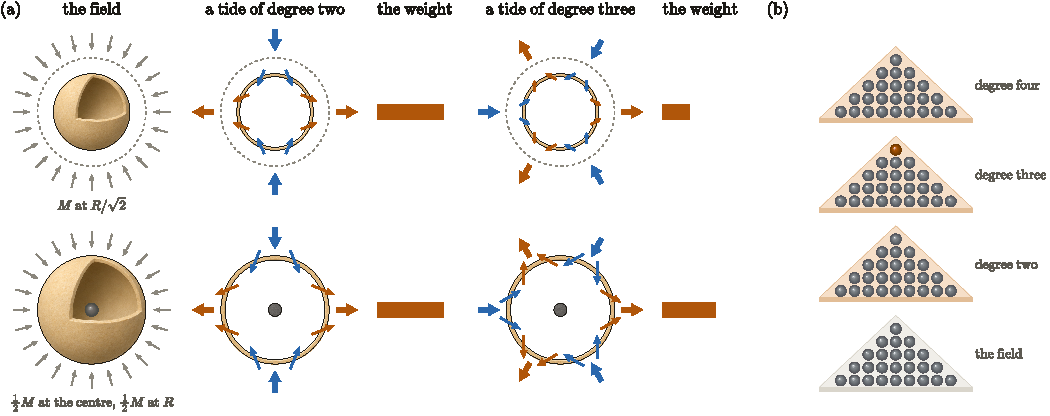
\includegraphics[width=\textwidth]{figures/ladder.pdf}
\caption{What a tide of a given degree reaches. (a) Two bodies with the same
field outside the radius $R$ (dotted): a thin shell of mass $M$ and radius
$R/\sqrt2$ (above), and a point of mass $M/2$ at the centre of a shell of
radius $R$ that holds the other half (below). Grey arrows: the pull outside
$R$, the same for both. The impulses of a tide of profile $(x^2 - y^2)/2$ and
of one of profile $(x^3 - 3xy^2)/3$, outward (orange) or inward (blue), are
drawn on sections of the two; the bars are the energies gained,
$\tfrac12\epsilon^2$ times $MR^2/3$ for both under the first, and
$\tfrac{2}{15}\,MR^4$ and $\tfrac{4}{15}\,MR^4$ under the second. (b) The
moments that are reached, a bead for each as in Fig.~\ref{fig:hair}(b), the
$2\ell + 1$ of each degree $\ell$ in a row. The field at one time holds the
lowest floor, $\int\rho\,r^\ell Y_\ell\,\dd V$; tides of degree two add the
next, with $r^{\ell+2}$, and each further degree one floor more,
Eq.~\eqref{eq:ladder}. The orange bead, $\int\rho\,r^4\,\dd V$, is the first at
which the two bodies differ. The cutaway bodies are pictures, and the skins and
the mass at the centre are drawn with some size.}\label{fig:ladder}
\end{figure*}

\paragraph{The flow.} The same measurements, carried one order further in the
time between the tide and the reading, give the motion inside the body. The
rates of change of two moments have the bracket
\begin{equation}\label{eq:flow-bracket}
\{\dot Q_h, \dot Q_g\} = \int\mathbf J\cdot\bigl[(\nabla\nabla h)\,\nabla g
- (\nabla\nabla g)\,\nabla h\bigr]\,\dd V ,
\end{equation}
with $\mathbf J$ the density of momentum and $\nabla\nabla h$ the matrix of
second derivatives. It is the part of the response that changes sign when the
profile applied and the moment read are exchanged: to second order in a short
time $\tau$, the change of $Q_h$ per unit of a weak impulse of profile $g$, less the
change of $Q_g$ per unit of one of profile $h$, is $\tau^2\{\dot Q_h, \dot Q_g\}$.
For the pair $h_\pm$ of Eq.~\eqref{eq:calderon} the bracket is
$-\tfrac12|\boldsymbol\xi|^2\,\boldsymbol\eta\cdot\tilde{\mathbf J}(\boldsymbol\xi)$,
with $\tilde{\mathbf J}$ the Fourier transform of the flow. Turning
$\boldsymbol\eta$ about $\boldsymbol\xi$ gives both components across
$\boldsymbol\xi$, and the rate of change of the density gives the third. The
flows that have no magnetic field outside (Section~\ref{sec:near-field}) are
therefore read from outside as the density is. The sphere of that section
whose inner part turns one way and its outer part the other, with no angular
momentum and no magnetic field outside it, is an example
(Fig.~\ref{fig:hidden-flow}). For quadrupolar
profiles the bracket is proportional to the angular momentum, and vanishes.
For the octupolar pair $h + ig = (x + iy)^3/3$ it is
\begin{equation}\label{eq:hidden-spin}
\{\dot Q_h, \dot Q_g\} = \tfrac{32}{35}\bigl(1 - 2^{-2/5}\bigr)\,M\Omega R^4
= 0.221\,M\Omega R^4 ,
\end{equation}
with $\Omega$ the rate of turning, and it changes sign with the sense of the
turning. In a trapped gas the same bracket, divided by the sum of
Eq.~\eqref{eq:sum-rule}, is the splitting of the quadrupole modes by a vortex
\cite{ZambelliStringari1998}.

\begin{figure}
\centering
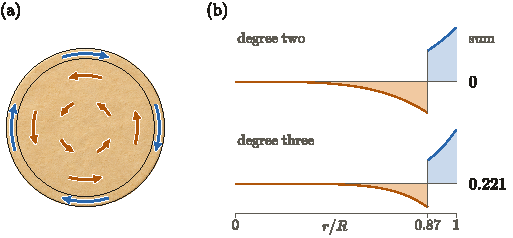
\includegraphics[width=\columnwidth]{figures/hidden-flow.pdf}
\caption{A flow that the exterior field does not show, and what two tides
read of it. (a) A uniform sphere in section through its equator, seen along
the axis about which it turns: the inner ball, out to $2^{-1/5}$ of the
radius, turns one way (orange) and the rest the other (blue), at the same
rate, so that the sphere has no angular momentum and no magnetic field
outside. Each arrow is the path of a part in one interval of time. (b) The
share of each radius in the bracket of Eq.~\eqref{eq:flow-bracket}, for the
pairs of profiles $h + ig = (x + iy)^n/n$ with $n = 2$ and $3$, each drawn to
its own greatest value. The inner ball counts with one sign and the rest with
the other, in proportion to $r^{2n}$. For degree two the two areas are equal,
as they are in the angular momentum, and the sum is zero. For degree three the
outer part counts for more, and the sum is $0.221\,M\Omega R^4$,
Eq.~\eqref{eq:hidden-spin}. The stone of the section is a
picture.}\label{fig:hidden-flow}
\end{figure}

\paragraph{The algebra of the moments and the energy.} The result can be stated
algebraically. A
quantity whose Poisson bracket with every harmonic moment vanishes does not
depend on the momenta, and if its bracket with the energy vanishes too it is a
constant (Appendix~\ref{app:proofs}). In this sense the moments and the weight, all of them
measured outside, generate all that can be determined of the body; the moments
alone leave every function of position undetermined. The moments are
themselves generators. In general relativity the mass moments are the charges
of the transformations $f\,\partial_t + t\,\nabla f\cdot\nabla$
with $f$ harmonic, which are the translation in time for $f = 1$
and the boosts for $f$ linear \cite{CompereOliveriSeraj2018}; those of
higher degree do not close under the bracket of vector fields, and their
algebra was left open. For matter it follows from the brackets of the energy
density \cite{Dirac1962,Schwinger1963}. To order $1/c^2$ the moments of the
energy do not commute among themselves,
\begin{equation}\label{eq:moment-bracket}
\{Q_h, Q_g\} = \frac{1}{c^2}\int\mathbf J\cdot(g\,\nabla h - h\,\nabla g)\,\dd V .
\end{equation}
For two dipoles this is $-L_z/c^2$, the bracket of the mass dipoles
\cite{Pryce1948}. For the quadrupoles $x^2 - y^2$ and $2xy$ it is
$-(2/c^2)\int(x^2 + y^2)\,\ell_z\,\dd V$, with $\ell_z$ the density of angular
momentum about the $z$ axis: a moment of the flow that the exterior field does
not hold, and one that does not vanish for the sphere of
Eq.~\eqref{eq:hidden-spin}. In general relativity, where the
energy is itself a term at the boundary, the corresponding statement was made by Marolf
\cite{Marolf2009,Marolf2014}, who noted that it does not by itself let a classical
observer determine the interior from the boundary:
$L_z$ is the bracket of
$L_x$ and $L_y$, yet the values of those two do not determine $L_z$; Jacobson
and Nguyen trace the failure of the argument for classical fields to a lack of
analyticity in time \cite{JacobsonNguyen2019}. This holds
for an observer who only measures the field. An observer who can apply a tide
measures brackets, since the bracket of two quantities is the response of the
first to an impulse generated by
the second, and Eq.~\eqref{eq:push} is such a response taken twice. If the body
is warm no tide need be applied: its thermal motion supplies the impulses, and in the
classical tremor, $\langle\dot Q_h\dot Q_g\rangle = k_BT\int\rho\,\nabla h\cdot\nabla g\,\dd V$,
the temperature stands where $\hbar$ stands in
Eq.~\eqref{eq:hair-commutator}. In quantum mechanics the zero-point motion
supplies them at any temperature, which is why the correlations of
a quantum state contain its commutators, and a cold classical body's do not.

\section{A black hole under a tide}\label{sec:hole}

\begin{quote}
\textbf{In plain words.} A black hole yields to a tide, as a body does, and
the yielding can be weighed in the same way. Weighed with one shape of tide,
it looks like a shell of its own mass just outside its edge. Weighed with
three, it looks like nothing that could be made of matter.
\end{quote}

\paragraph{The response of a black hole to a tide.} A black hole responds to a tide as no ordinary body does.
Its Love numbers are zero \cite{BinningtonPoisson2009,DamourNagar2009}, with
spin as without \cite{CharalambousDubovskyIvanov2021}: a steady tide raises no
moment on a hole that does not turn, and on one that turns it raises one by
friction only, since a tide that is not symmetric about the axis of spin is
not steady to the turning horizon. In
a tide that changes slowly a hole of mass $M$ and Schwarzschild radius $r_s$,
not turning, absorbs energy at the rate \cite{Poisson2004}
\begin{equation}\label{eq:horizon-friction}
\begin{gathered}
\frac{\dd E}{\dd t} = \nu\,\bigl(\dot{\tE}_{ij}\dot{\tE}_{ij}
+ \dot{\tB}_{ij}\dot{\tB}_{ij}\bigr),\\
\nu = \frac{16}{45}\,\frac{G^5M^6}{c^{13}} = \frac{M r_s^5}{90\,c^3} ,
\end{gathered}
\end{equation}
so that its quadrupole $Q_{ij}$, defined by the energy $Q_{ij}\tE_{ij}$ in a
tide (half of Newton's $\int\rho\,(x_ix_j - \tfrac13r^2\delta_{ij})\,\dd V$),
responds with $\mathrm{Im}\,\chi = \nu\omega$ and no elastic part
\cite{GoldbergerRothstein2006}. This is the
absorption of long gravitons, seen in the near field: through that coupling
and its magnetic counterpart, which the horizon answers with the same friction,
the limit of Section~\ref{sec:vistas} for the absorption of a quadrupole wave is
$(16/5)\,G\nu\,\omega^6/c^5$ \cite{GoldbergerRothstein2020}.

\paragraph{The fluctuations of a black hole's quadrupole.} For a hole formed by
collapse and left alone, that quadrupole also fluctuates, at frequencies far below
$c/r_s$, with a flat spectrum \cite{GoldbergerRothstein2020}:
\begin{equation}\label{eq:hole-noise}
\begin{gathered}
\langle Q_{ij}(t)\,Q_{kl}(0)\rangle
= \Pi_{ijkl}\int S_Q\,e^{-i\omega t}\,\frac{\dd\omega}{2\pi},\\
S_Q = \frac{\hbar\,r_s^5}{360\pi G} ,
\end{gathered}
\end{equation}
with $\Pi_{ijkl} = \tfrac12(\delta_{ik}\delta_{jl} + \delta_{il}\delta_{jk})
- \tfrac13\delta_{ij}\delta_{kl}$. The spectrum was found by matching to Hawking's radiation, for which at
these frequencies the chance of emitting a quantum and the chance of absorbing
one are both the classical absorption times $k_BT/\hbar\omega$. Inserting
Eqs.~\eqref{eq:horizon-friction} and~\eqref{eq:hole-noise} into the thermometer
of Eq.~\eqref{eq:thermometer} gives
\begin{equation}\label{eq:hole-thermometer}
T = \frac{S_Q}{2k_B\,\nu} = \frac{\hbar c^3}{8\pi G M k_B} ,
\end{equation}
the Hawking temperature. The result is not independent, the noise
having been fixed by matching to radiation at that temperature; what it confirms
is that the friction, found from the growth of the horizon, and the absorption,
found from the scattering of waves, are the same number. A hole's near field
therefore obeys the rule of every warm body, noise equal to
friction at its own temperature, so that a camera beside it reads that
temperature from the field that does not radiate, without absorbing any quantum of
the radiation. The signal is far beyond reach, like most in this
paper: for a hole as warm as the graviton sky, $0.905\,\mathrm{K}$, it is
$4\times10^{-32}\,\mathrm{s^{-2}}$ in a second, a metre away, where the hole's
steady tide is $2\times10^{13}\,\mathrm{s^{-2}}$. The tremor carries nothing
else. A stone's tremor carries $\int\rho\,\nabla h\cdot\nabla g\,\dd V$ for
every pair of harmonic functions, and so the whole of its interior; a hole's
carries $M$ again (Table~\ref{tab:hair}).

\paragraph{The weight of a black hole's response.} For ordinary matter the sum
of Eq.~\eqref{eq:sum-rule} is the inertia that a tide has to move: for a round
body under a quadrupolar tide, $\tfrac13\int\rho\,r^2\,\dd V$. The response of
a hole can be weighed in the same way. At any frequency its dissipative part
is fixed by the fraction $\Gamma_2$ of a quadrupole wave that the hole
absorbs, $\mathrm{Im}\,\chi = 5c^5\Gamma_2/16G\omega^5$, of which
Eq.~\eqref{eq:horizon-friction} is the limit at low frequency. With $\Gamma_2$
found from the Regge--Wheeler equation, and $x = GM\omega/c^3$,
\begin{equation}\label{eq:hole-sum-rule}
\begin{aligned}
\frac{2}{\pi}\int_0^\infty\omega\,\mathrm{Im}\,\chi\,\dd\omega
&= \frac{5}{32\pi}\,Mr_s^2\int_0^\infty\frac{\Gamma_2}{x^4}\,\dd x\\
&= 0.345\,Mr_s^2 .
\end{aligned}
\end{equation}
A round body of the hole's mass has this sum if its mass lies at a
root-mean-square radius of $1.02\,r_s$: to a changing quadrupolar tide a hole that does
not turn has the inertia of a shell of its own mass just outside its horizon
(Fig.~\ref{fig:hole-response}(b)).
The same sum can be taken for the tide of every degree. For a round body each
tide of degree $\ell$ gives $\int\rho\,r^{2\ell-2}\,\dd V$,
Eq.~\eqref{eq:thermal-multipole}, and the sequence fixes the density at every
radius. For the hole, written as the radius of the shell of its own mass that
has the same sum, they are $1.02$, $1.46$, $1.61$, $1.69$ and $1.73\,r_s$ for
$\ell = 2$ to $6$, and tend to $(3\sqrt3/e)\,r_s = 1.91\,r_s$ (Fig.~\ref{fig:hole-response}(c)). No body has
these sums. For any distribution of positive mass
$\int\rho\,r^2(r^2 - a)^2\,\dd V$ cannot be negative, and with the hole's sums
for $\ell = 2$, $3$ and $4$ it is $-2.04\,Mr_s^6$ at $a = 4.34\,r_s^2$. Read
through the conversion that holds for every body, the absorption of a black
hole is therefore the tidal inertia of no distribution of positive mass: one
tide lets it be drawn as a shell, and three allow no drawing. The moments in
frequency of the response to one tide are those of a positive measure
\cite{KehagiasRiotto2026}; it is the sums across the degrees that belong to no
body. Any absorber
that takes all that comes within a fixed radius fails in the same way, and no
matter does that to a gravitational wave (Sections~\ref{sec:thermal}
and~\ref{sec:no-lens}).
The same absorption, put into the dispersion relation that holds for matter,
$\chi(0) = (2/\pi)\int\mathrm{Im}\,\chi\,\dd\omega/\omega$, would give a body
of radius $r_s$ the Love number $k_2 = 1.35$ in the convention of Section~\ref{sec:near-field}, and the hole's is zero. That the
relation cannot hold for a hole without a subtraction, and that a term local
in time cancels the dispersive part of its static response, are known
\cite{Porto2016,GoldbergerLiRothstein2021,KehagiasRiotto2026}; the two numbers
give the sizes.

\begin{figure}
\centering
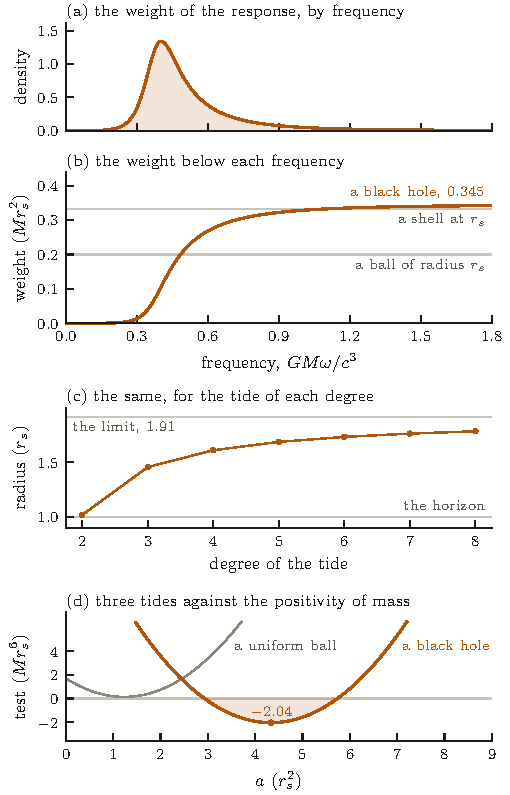
\includegraphics[width=\columnwidth]{figures/hole-response.pdf}
\caption{The weight of a black hole's response to a tide. (a) The integrand
of Eq.~\eqref{eq:hole-sum-rule}, $(5/32\pi)\,\Gamma_2/x^4$ with
$x = GM\omega/c^3$, in units of $Mr_s^2$. It is greatest at $x = 0.40$. (b) Its
sum below each frequency, which tends to $0.345\,Mr_s^2$. The lines are the
sums of two round bodies of the hole's mass,
$\tfrac13\int\rho\,r^2\,\dd V$: a thin shell of radius $r_s$ and a uniform
ball of that radius. (c) The same sum for the tide of each degree, as the
radius of the shell of the hole's mass that has it. The radii tend to
$(3\sqrt3/e)\,r_s$, and the first three belong to no distribution of positive
mass.}\label{fig:hole-response}
\end{figure}

\begin{table*}
\centering
\begin{tabular}{p{0.2\textwidth}p{0.4\textwidth}p{0.34\textwidth}}
 & A stone, a planet, a star & A black hole \\ \hline
The field at one time & the harmonic moments of its mass and its flow & at rest, mass, place and spin: seven numbers \\
Bits, at $\SNR$ & $[L^3/3\Lambda^2 + L^2/2\Lambda]/\ln 2$ & $7\log_2\SNR$ \\
A steady tide & its Love numbers & nothing, if it does not turn \\
A changing tide & when fast, $-\omega^{-2}\int\rho\,\nabla h\cdot\nabla g\,\dd V$: the density & when slow, friction, $\nu$ \\
Tides of degree up to $m$ & the moments $\int\rho\,r^{\ell+2j}Y_\ell\,\dd V$ with $j < m$ & nothing more \\
The sums, tide by tide & $\int\rho\,r^{2\ell-2}\,\dd V$: the density of a round body & the moments of no distribution of positive mass \\
A mass that passes & its own loss of energy, $\tfrac12C^2\int\Sigma\,|\mathbf b - \mathbf s|^{-2}\,\dd^2s$: the density & what the hole absorbs, set by its mass and spin \\
Two tides, in either order & $\{\dot Q_h, \dot Q_g\}$: the flow & nothing more \\
Its tremor & $\langle\dot Q_h\dot Q_g\rangle = k_BT\int\rho\,\nabla h\cdot\nabla g\,\dd V$: the density, at a known temperature & $S_Q = 2k_BT\nu$ at low frequencies: the temperature \\
Its weight, after a tide & after an impulsive one, $\tfrac12\epsilon^2\int\rho\,|\nabla g|^2\,\dd V$ more: the density & after a slow one, $\nu\int(\dot{\tE}_{ij}\dot{\tE}_{ij} + \dot{\tB}_{ij}\dot{\tB}_{ij})\,\dd t$ more: its mass \\
\end{tabular}
\caption{What the field outside a body determines of its interior, for ordinary matter
and for a black hole. $L = \ln\SNR$ and $\Lambda = \ln(R_c/R)$ are those of
Eq.~\eqref{eq:hair-bits}; $h$ and $g$ are harmonic functions; $\nu$ is the
horizon's friction, Eq.~\eqref{eq:horizon-friction}; in the last line the
stone's entry is Eq.~\eqref{eq:push}, and the hole's holds for a tide that
changes little in the time $r_s/c$.}\label{tab:hair}
\end{table*}

\section{What remains of holography}\label{sec:holography}

\begin{quote}
\textbf{In plain words.} It has been argued that in quantum gravity everything
inside a region can be learnt at its edge. In ordinary physics a weaker thing
is true, and it can be said exactly. The pull of a body, read on a surface
around it, holds a surface's worth of what is inside, and no more. The rest
can still be had from outside, but not by looking: something must be done to
the body, and the energy counted afterwards.
\end{quote}

\paragraph{Black holes and the classical limit.} For ordinary matter, then,
the exterior field determines the interior, with a precision that grows as the
logarithm of the sensitivity. The statement is one about operations. For a
given class of bodies, and given tides, moments and times, either two
interiors are told apart or every allowed measurement gives the same result
for both, and Eqs.~\eqref{eq:split} and~\eqref{eq:ladder} say which. For a black hole the exterior field gives seven
numbers at one time, in the frame in which it is at rest, and a temperature at
two; a hole subjected to a slow tide and then weighed has gained
$\nu\int(\dot{\tE}_{ij}\dot{\tE}_{ij} + \dot{\tB}_{ij}\dot{\tB}_{ij})\,\dd t$,
which gives its mass again, and whatever the tide, what it gains is set by its
mass and spin alone. Whether the exterior field holds more is the question of the fate of
what falls in. It has been argued that in quantum gravity it does:
that everything massless particles will carry out to infinity can be learnt
there before they arrive, from correlations of the energy with the waves
\cite{LaddhaEtAl2021}; that observers at the boundary of an asymptotically
anti-de Sitter space can find the state within by simple operations there and
a measurement of the energy \cite{ChowdhuryPapadoulakiRaju2021}; that the
state of a single particle can be reconstructed from the metric at spatial
infinity, through its momentum and its centre of energy \cite{Donnelly2018};
and that
quantum corrections to the field outside an ordinary body depend on its
density profile where the classical field does not \cite{CalmetEtAl2022}.
The first two are said by their authors to have no classical counterpart, and
for a reading at one time they have none, by Newton's shell theorem. Counted at
a resolution $d$, the harmonic moments held by a surface of radius $R$ number
$(R/d)^2$ against the $(R/d)^3$ cells within it.
An impulsive tide followed by a weighing is what remains of the first two
without $\hbar$:
an operation made from
outside and then a reading of the energy. Its differences from the quantum
results show what in them is quantum. It needs time, for the tide to reach the
body and the change of mass to be read, where
they need next to none. It gives a density and a motion, not a state. It is not
peculiar to gravity, since the work done by any applied force can be measured, and
charges obey the analogue of Eq.~\eqref{eq:push} with the square of the charge
over the mass in place of the mass; what is peculiar to gravity is that no part
of a body can be shielded from the tide, that the quantity read is the mass itself, and that the
result remains in the field outside. On a black hole the method
fails. A hole's tremor is of order $\hbar$, its temperature in
Eq.~\eqref{eq:hole-thermometer} being proportional to it: without $\hbar$ a
hole is at zero temperature and has no tremor, and under a tide it gives only its mass. Whatever more the
exterior field holds of a hole is of order $\hbar$, beyond the classical
account given here.

\paragraph{What gravity cannot decohere.} The null space has a meaning in
quantum mechanics. Put a body into a superposition of two arrangements of its
mass that have the same field outside: a ball and a shell, the nugget and its
skin, or two stages of any motion that keeps a body round. At any one time the
field outside is the same in both branches, if they have the same energy. It holds no record of which, and
nothing outside that touches the body through its field alone can learn which
from a reading at one time; if the superposition is made by a motion that leaves the field
outside unchanged throughout, as a round motion does, no graviton is emitted in
making it. To the outside the branches differ only in readings at two times, in their
tremor and in their response to a tide, Eq.~\eqref{eq:dust}. Yet they differ at
once in the measure by which Di\'osi
and Penrose proposed that gravity itself ends superpositions
\cite{Diosi1987,Penrose1996}, the gravitational self-energy of the difference
of the two densities:
\begin{equation}\label{eq:dp-energy}
E_G = \frac{1}{8\pi G}\int|\mathbf g_1 - \mathbf g_2|^2\,\dd V = \frac{GM^2}{10R}
\end{equation}
for a ball and a shell of mass $M$ and radius $R$, whose fields
$\mathbf g_{1,2}$ differ only inside (the numerical factor in front of $E_G$ is
a matter of convention). For the mass and size of a glass bead a micrometre in
radius, $\hbar/E_G$ is a fifth of a second; a real bead cannot move its mass to
its surface, and if it only breathes, by a part $\delta/R$ of its radius,
$E_G = \tfrac{9}{10}(\delta/R)^2GM^2/R$ and the time is longer by
$R^2/9\delta^2$. Such a pair would separate two ways in which gravity might end
a superposition. The ordinary way, by carrying away a record of it
\cite{Belenchia2018,DanielsonSatishchandranWald2022}, is closed (save for
tides from outside, which the branches answer differently, Eq.~\eqref{eq:dust},
at second order in the coupling), and a collapse
of Di\'osi's and Penrose's kind is not (in its simplest form, with no free
length, it has since been excluded by experiment \cite{DonadiEtAl2021}). A spherical
disturbance with no change of mass has been noted, for dark matter, to be the
kind most robust against decoherence by gravity \cite{AllaliHertzberg2020}.
